% kappa.tex
% STOLAR: Form Follows Fitness
% Kappa-tekst for artikkelbasert avhandling
% Spraak: Nynorsk

\documentclass[12pt, a4paper]{article}

\usepackage[utf8]{inputenc}
\usepackage[T1]{fontenc}
\usepackage[nynorsk]{babel}
\usepackage{mathpazo}
\usepackage{amsmath, amssymb}
\usepackage{booktabs}
\usepackage{graphicx}
\usepackage{xcolor}
\usepackage{hyperref}
\usepackage[round]{natbib}
\usepackage{setspace}
\usepackage{geometry}
\usepackage{csquotes}
\usepackage{float}
\usepackage{enumitem}

\geometry{margin=2.5cm}
\onehalfspacing
\graphicspath{{fig/}}

\title{%
  \vspace{-2cm}
  {\large Arkitektur- og designhøgskolen i Oslo}\\
  {\large Institutt for design}\\[2cm]
  {\Huge\textbf{STOLAR}}\\[0.5em]
  {\LARGE Form Follows Fitness}\\[0.5em]
  {\large Kvantitativ analyse av europeisk stoldesign, 1280--2024}\\[3cm]
  {\normalsize Iver Raknes Finne}\\[0.5em]
  {\small Masteroppgåve i design}\\
  {\small Våren 2026}\\[1em]
  {\small Rettleiar: [rettleiarnamn]}
}
\author{}
\date{}

\begin{document}
\maketitle
\thispagestyle{empty}
\newpage

% ================================================================
\begin{abstract}
\noindent Denne avhandlinga undersøkjer empirisk om Louis Sullivan sitt aksiom ``form ever follows function'' held mot eit reelt datasett. Gjennom kvantitativ analyse av 2\,284 stolar frå Nasjonalmuseet for kunst, arkitektur og design og Victoria \& Albert Museum, registrerte mellom 1280 og 2024, byggjer avhandlinga ein kumulativ beviskjede over fire artiklar.

\emph{Artikkel~I} avdekkjer at materialar ikkje er nøytrale medium, men komprimerte geopolitiske historier: Shannon-entropien stig monotont frå $H' = 1{,}0$ til 5,07 bits over 700 år. \emph{Artikkel~II} viser at dimensjonar driftar under geografisk og teknologisk påverknad, med systematisk negative Modulor-avvik ($-18$ til $-40$ cm). \emph{Artikkel~III} demonstrerer at dimensjonar og materialkombinasjonar predikerer stilperiode med $F1 = 0{,}823$ og nasjonalitet med $F1 = 0{,}721$, medan stilmerket åleine er den svakaste prediktoren for faktisk geometri. \emph{Artikkel~IV} samlar bevisa og formulerer \textbf{Form Follows Fitness} (FFF) som eit koherent alternativ: form er ikkje dedusert frå funksjon, men selektert av eit fleirdimensjonalt tilpassingslandskap der materiale, teknologi, økonomi, geografi og kultur alle utøver seleksjonstrykk.

Kappa-teksten syntetiserer beviskjeda, demonstrerer at FFF er eit paradigmeskifte i Kuhn sin tyding, og viser at rammeverket generaliserer frå stolar til alle estetiske fag. Ein proposisjonell traktat formaliserer dei sju kardinale prinsippa i FFF.

\medskip
\noindent\textbf{Nøkkelord:} Form Follows Fitness, fitnesslandskap, stoldesign, kvantitativ designhistorie, materialaffordanse, seleksjonstrykk, Shannon-entropi
\end{abstract}

\newpage
\tableofcontents
\newpage


% ================================================================
\section{Innleiing: ein revolusjon i fire akter}

\begin{quote}
``It is the pervading law of all things organic and inorganic [\ldots] that \emph{form ever follows function}. This is the law.'' \citep{sullivan1896}
\end{quote}

\subsection{Bakgrunn og motivasjon}

I over eit hundreår har Louis Sullivan sitt aksiom fungert som grunnlova i formgjevingsfaga. \citet{lecorbusier1923} bygde ein arkitektonisk doktrine på premissen. \citet{alexander1964} foreslo systematisk formderivering frå funksjonskrav. \citet{giedion1948} dokumenterte mekaniseringa. Ingen stilte spørsmålet empirisk.

Denne avhandlinga stiller det. Metoden er enkel: samle alle stolar med same funksjon, måle dei, og sjå om formvariasjonen er liten nok til å støtte aksiomet. Ho er ikkje det.

\subsection{Datamaterialet}

STOLAR-databasen inneheld 2\,284 stolar frå to europeiske museumssamlingar: Nasjonalmuseet for kunst, arkitektur og design (NMK) i Oslo ($n = 671$), og Victoria \& Albert Museum (V\&A) i London ($n = 1\,613$). Tidsrommet strekkjer seg frå 1280 til 2024. Alle objekta deler same invariante funksjon: å bere ein sitjande kropp.

Kvar stol er dokumentert med dimensjonsvariablar (høgde, breidde, djupn, setehøgde), materiallister, teknikkar, stilmerke (22,9\,\% dekning), nasjonalitet (70,2\,\% dekning) og produksjonsår.

\subsection{Forskingsspørsmål}

Avhandlinga stiller fem spørsmål:
\begin{enumerate}
  \item Er formvariasjonen stor nok til å falsifisere funksjonsdeterminismen?
  \item Kva seleksjonstrykk forklarer mest formvariasjon?
  \item Er stilperiode ei årsak til form, eller eit emergent restprodukt?
  \item Korleis endrar tilpassingslandskapet seg over tid?
  \item Kan ein formulere eit empirisk testbart alternativ til funksjonalismen?
\end{enumerate}

\subsection{Avhandlingsstruktur}

Avhandlinga er artikkelbasert. Fire artiklar utgjer beviskjeda; denne kappa-teksten syntetiserer dei til ei samanhengande forteljing og presenterer det overordna teoretiske rammeverket, Form Follows Fitness. Kapittel~2 etablerer det teoretiske fundamentet. Kapittel~3 beskriv metoden. Kapittel~4 samanfattar kvar artikkel. Kapittel~5 presenterer den overordna syntesen. Kapittel~6 inneheld traktaten. Kapittel~7 konkluderer.


% ================================================================
\section{Teoretisk rammeverk: fem pilarar}

Rammeverket Form Follows Fitness kviler på fem tverrvitskaplege pilarar. Ingen av dei er nye i seg sjølve; det nye er syntesen.

\subsection{Fitnesslandskapet}

\citet{wright1932} introduserte omgrepet \textbf{fitnesslandskap} som ein topografisk modell av evolusjonær tilpassing. \citet{kauffman1993} utvida modellen til komplekse system med fleire lokale optimum. I FFF er forma ein posisjon i eit $n$-dimensjonalt landskap der kvar akse representerer eit seleksjonstrykk. Stilar er lokale toppunkt: mellombels stabile formkonfigurasjonar som overlever så lenge landskapet ikkje endrar seg.

\subsection{Distribuert kognisjon}

\citet{clark2008} formulerte den utvida kognisjonshypotesen. \citet{levin2019} utvida dette til ein generell teori om kognisjon på alle skalaer. I FFF tyder dette at materialet ``veit'' kva det toler, verktøyet avgrensar formrommet, og marknaden selekterer.

\subsection{Utforsking og utnytting}

Avveginga mellom \textbf{exploration} og \textbf{exploitation} er formalisert i forsterkingslæring \citep{sutton2018} og i paleontologien som \textbf{punctuated equilibrium} \citep{eldredge1972}. Designhistoria vekslar mellom desse to fasane: lange periodar med utnytting der forma konvergerer, avbrotne av raske utforskingsfasar utløyste av teknologiske eller geopolitiske sjokk.

\subsection{Affordanse}

\citet{gibson1977} definerte \textbf{affordanse} som dei handlingsmoglegheitene eit miljø tilbyr ein organisme. \citet{pye1968} skilde mellom ``the workmanship of risk'' og ``the workmanship of certainty''. I FFF yter kvart materiale ei distinkt form for tilbod og motstand, ein affordanse som fysisk kanaliserer bestemte geometriar og stengjer andre ute.

\subsection{Morforom}

\citet{raup1966} introduserte \textbf{morphospace}: det teoretiske rommet av alle moglege former ein biologisk struktur kan innta. I FFF er formrommet analogt: totaliteten av alle moglege geometriske, materielle og operasjonelle tilstandar. Dei tome regionane fortel kva former som er fysisk, teknologisk eller kulturelt umoglege.

\subsection{Sullivan som degenerert spesialtilfelle}

``Form follows function'' er logisk gyldig berre når alle seleksjonstrykk utanom funksjon er eksakt lik null. Fellesinformasjonsanalysen (figur~\ref{fig:mi}) syner at funksjon ber \emph{null} informasjon om stilperiode (MI = 0,000 bits), medan proporsjonar ber 2,072 bits, tid 1,546 bits, og materiale 1,456 bits. Funksjonalismen er eit degenerert spesialtilfelle.

\begin{figure}[H]
  \centering
  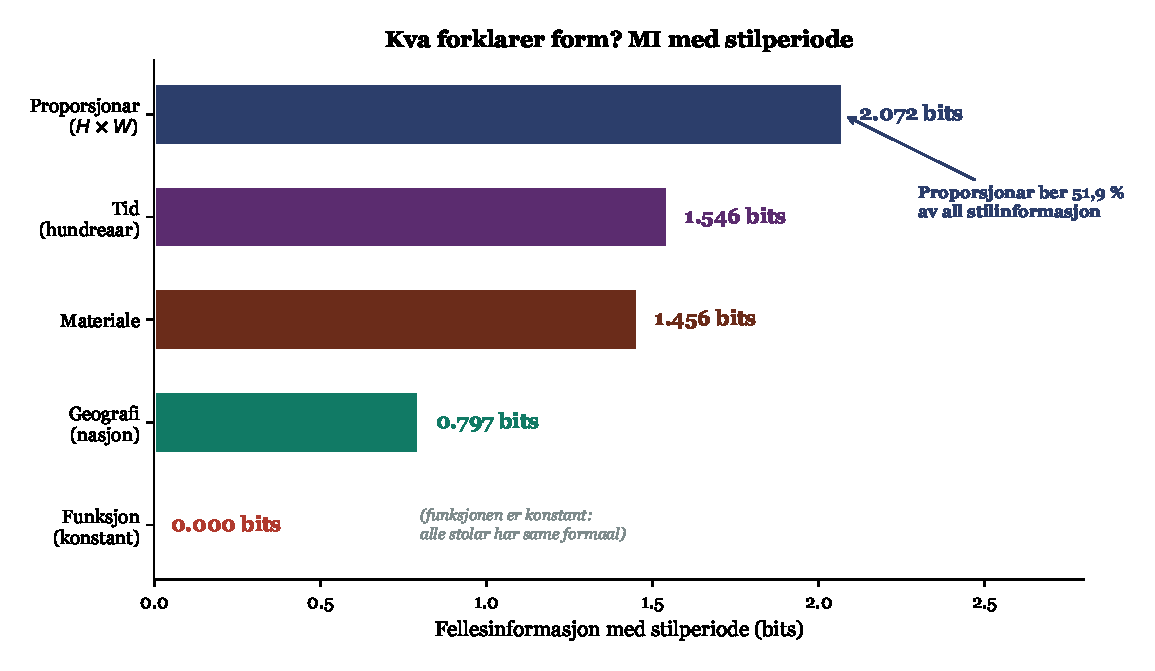
\includegraphics[width=\textwidth]{fig15_mi_stil.pdf}
  \caption{Fellesinformasjon med stilperiode. Proporsjonar ber 51,9\,\% av all stilinformasjon. Funksjon ber null.}
  \label{fig:mi}
\end{figure}


% ================================================================
\section{Metode og datamateriale}

\subsection{Datainnsamling}

STOLAR-databasen vart bygd frå to kjelder. NMK-dataa ($n \approx 700$) vart henta frå Digitalt Museum (DiMu) sitt API og supplerte med manuell kontroll. V\&A-dataa ($n \approx 1\,600$) vart henta frå museet sitt opne API. Alle postar vart harmoniserte til eit felles skjema.

\subsection{Variablar}

\textbf{Dimensjonar:} Høgde, breidde, djupn, setehøgde (i cm). \textbf{Materialar:} Kommaseparerte lister, koda til 30 binære variablar for maskinlæring. \textbf{Teknikkar:} Kommaseparerte lister av konstruksjonsteknikkar. \textbf{Metadata:} Produksjonsår, stilperiode, nasjonalitet, museum.

\subsection{Statistiske metodar}

\begin{itemize}
  \item \textbf{Informasjonsteori:} Shannon-entropi ($H'$) og Pielou-jamnheit ($J'$) for å måle material- og teknikkmangfald over tid.
  \item \textbf{Klassifikasjon:} Random Forest (100 trær, 5-faldig stratifisert CV) for å predikere stilperiode, nasjonalitet og hundreår.
  \item \textbf{Avstandsmål:} Jaccard-avstand for materialsamanlikning mellom museum.
  \item \textbf{Effektstorleik:} Cohen's $d$ for dimensjonsskilnader mellom grupper.
\end{itemize}

\subsection{Avgrensingar}

Fire viktige atterhald: (1) Variablane er grove (fire lineære dimensjonar, ikkje fullstendig 3D-geometri). (2) V\&A dominerer datasettet. (3) Berre 22,9\,\% av objekta har stilmerke. (4) Museumssamlingar er ikkje representative populasjonar. Trass i desse avgrensingane er beviskjeda kumulativ og konvergent.


% ================================================================
\section{Dei fire artiklane}

\subsection{Artikkel I: Materialar som geopolitisk historie}

Den fyrste artikkelen introduserer \textbf{materialkurveanalyse} som metode. Shannon-entropien for materialar stig monotont frå $H' = 1{,}0$ bits (1200-talet, 2 materialar) til $H' = 5{,}07$ bits (1900-talet, 65 materialar). Analysen avdekkjer tre materialregime:

\begin{enumerate}
  \item \textbf{Det lokale treregimet} (1200--1500): bjørk, furu, eik. $H' < 2$ bits.
  \item \textbf{Det koloniale handelsregimet} (1600--1800): mahogni dominerer med opp til 17,3\,\% i V\&A. Jaccard-avstanden mellom NMK og V\&A fell frå 1,0 til 0,47.
  \item \textbf{Det industrielt-syntetiske regimet} (1900--2000): stål, kryssfiner, plast. Industrielle materialar når 32,3\,\%.
\end{enumerate}

Artikkelen innfører omgrepet \textbf{materiell dobbeltheit}: konstruksjonar der berande kjernar er lokalt tre, medan fasaden er importert edelt materiale. Fenomenet toppar med 23,5\,\% av stolane på 1800-talet.

\subsection{Artikkel II: Produksjonsgeografi og formkonvergens}

Den andre artikkelen undersøkjer korleis geografi og tid påverkar form. Gjennomsnittleg høgde fell frå 94,7 cm (1200-talet) til 73,1 cm (2000-talet), konsekvent 18--40 cm under Le Corbusier sin Modulor-prediksjon. $H/W$-ratioen driftar frå 1,68 til 1,37, vekk frå gullsnittet ($\varphi = 1{,}618$).

NMK-stolar er systematisk høgare enn V\&A-stolar i tidlege periodar ($\Delta = +24{,}6$ cm i 1600-talets gjennomsnitt), men skilnaden konvergerer mot null etter industrialiseringa, for deretter å divergere igjen i skandinavisk modernisme. Estimert medianvekt fell frå 20,4 kg til 6,8 kg.

\subsection{Artikkel III: Form og tid}

Den tredje artikkelen brukar maskinlæring for å teste kva variablar som kodar stil. Ein Random Forest-modell oppnår:

\begin{table}[H]
\centering
\begin{tabular}{@{}llc@{}}
\toprule
\textbf{Features} & \textbf{Mål} & \textbf{$F1$} \\
\midrule
Dimensjonar åleine & Stilperiode & 0,777 \\
Materialar åleine & Stilperiode & 0,678 \\
Dimensjonar + materialar & Stilperiode & 0,823 \\
Dimensjonar + materialar & Nasjonalitet & 0,721 \\
Dimensjonar + materialar & Hundreår & 0,776 \\
\bottomrule
\end{tabular}
\end{table}

Høgde er den viktigaste enkeltvariabelen (19,7\,\% feature importance). Teknikk-entropien stig parallelt med materialentropien, frå 1,0 til 3,67 bits. Stilperiodar er emergente merkelappar, ikkje kausale kategoriar.

\subsection{Artikkel IV: Form Follows Fitness}

Den fjerde artikkelen samlar åtte kumulative bevis, falsifiserer funksjonsdeterminismen, og formulerer FFF som eit testbart alternativ. Funksjonalismen er eit degenerert spesialtilfelle, gyldig berre når alle seleksjonstrykk utanom funksjon er null. Dette vilkåret er aldri oppfylt.


% ================================================================
\section{Syntese: frå fire artiklar til ein konklusjon}

\subsection{Beviskjeda}

Figur~\ref{fig:bevis} syner dei fire pilarane i beviskjeda.

\begin{figure}[H]
  \centering
  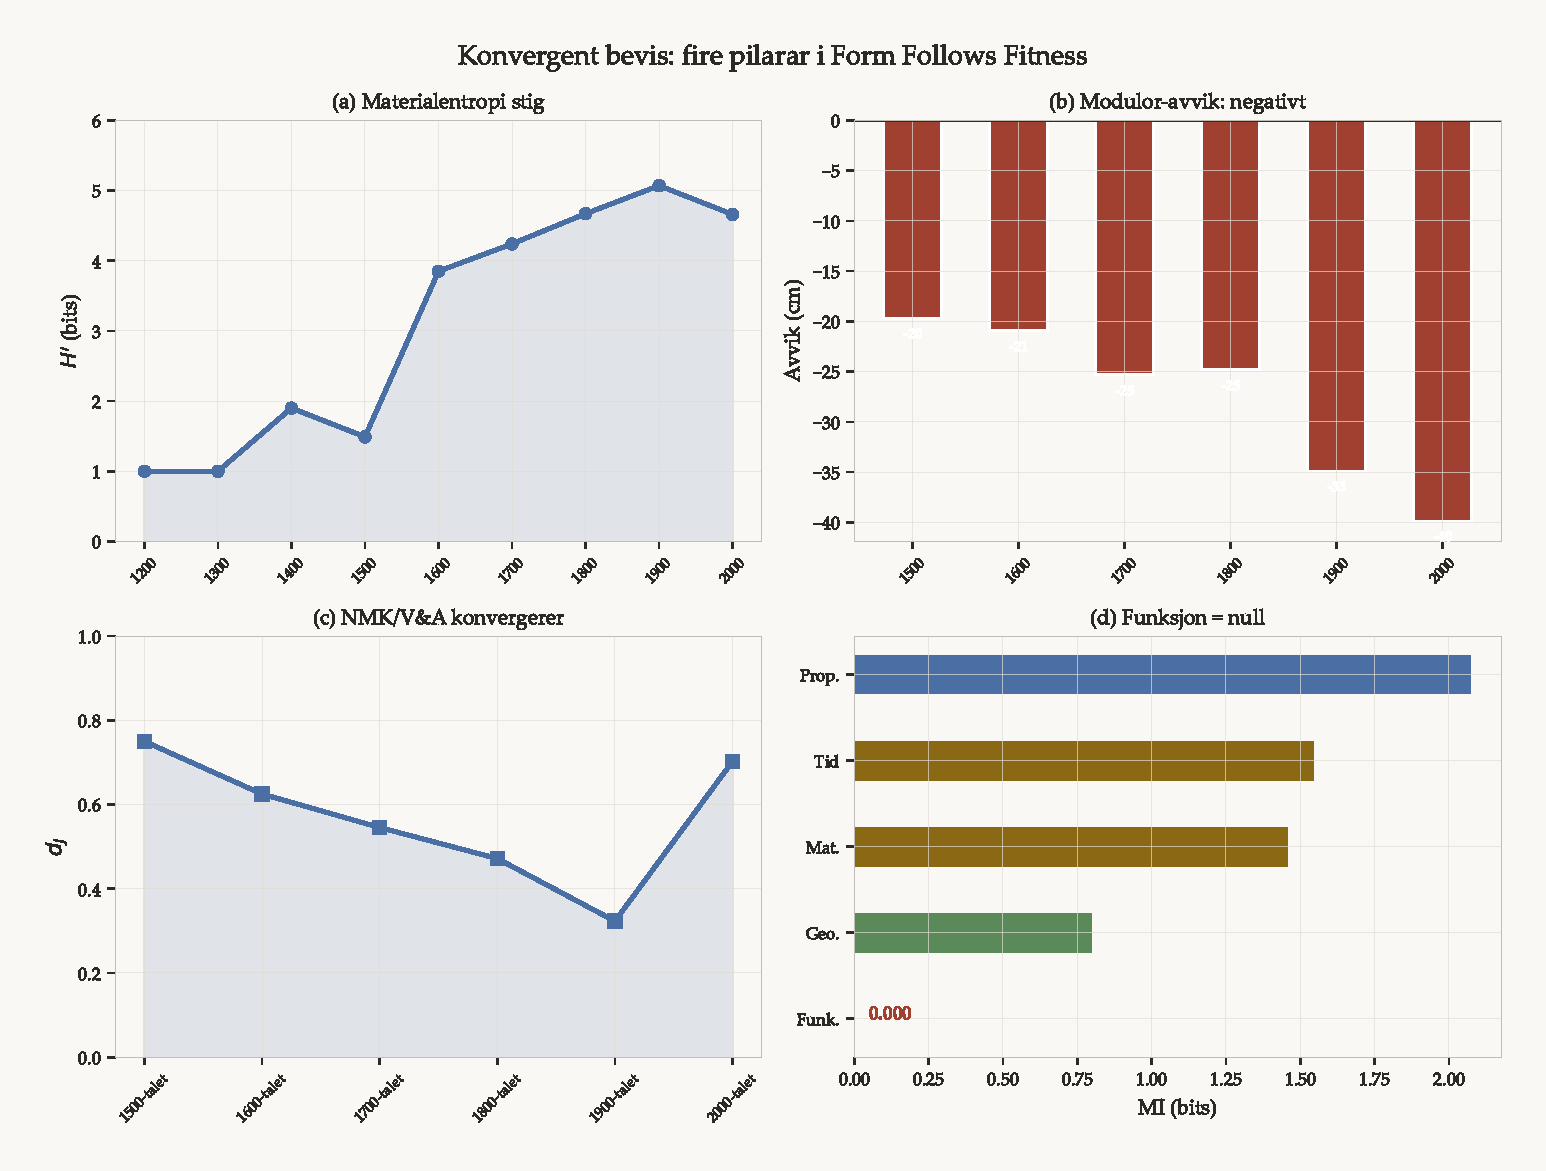
\includegraphics[width=\textwidth]{fig16_beviskjede.pdf}
  \caption{Konvergent bevis: (a) materialentropi stig monotont, (b) Modulor-avviket er systematisk negativt, (c) Jaccard-avstanden mellom NMK og V\&A konvergerer, (d) funksjon ber null informasjon om stil.}
  \label{fig:bevis}
\end{figure}

Dei fire artiklane byggjer ein kumulativ beviskjede:

\begin{itemize}
  \item \textbf{Artikkel~I} etablerer at materialar er agentiale substrat med eigne geopolitiske historier.
  \item \textbf{Artikkel~II} viser at form driftar under geografisk og teknologisk påverknad, ikkje konvergerer mot funksjonelt optimum.
  \item \textbf{Artikkel~III} demonstrerer at stilmerke er emergente restprodukt, ikkje årsaker.
  \item \textbf{Artikkel~IV} samlar bevisa og falsifiserer aksiomet.
\end{itemize}

\subsection{Paradigmeskifte}

\citet{kuhn1962} definerte eit paradigmeskifte som overgangen frå eitt sett av aksepterte normer til eit nytt. FFF oppfyller Kuhn sine kriterium på tre vis:

\begin{enumerate}
  \item \textbf{Anomali.} Funksjonalismen predikerer låg formvariasjon under konstant funksjon. Variasjonen er massiv.
  \item \textbf{Krise.} Postfunksjonalismen har kritisert aksiomet i 50 år, men utan å tilby eit kvantitativt, testbart alternativ.
  \item \textbf{Nytt paradigme.} FFF subsumerer funksjonalismen som eit degenerert spesialtilfelle og gjev eit rammeverk som er empirisk falsifiserbart, kvantitativt og substratuavhengig.
\end{enumerate}

\subsection{Generalisering}

FFF er utvikla på stolar, men rammeverket er substratuavhengig. Same logiske struktur gjeld for alle gjenstandar som (1) har ein invariant funksjon, (2) varierer i form, og (3) er utsette for fleire samverkande seleksjonstrykk. Arkitektur, bildesign, typografi, biologisk morfogenese og algoritmisk formgjeving lystrar alle same navigeringsmekanikk i eit tilpassingslandskap.


% ================================================================
\section{Traktat for form}

\noindent\emph{Det deterministiske aksiomet har falle. Her byrjar tilpassinga.}

\bigskip

\noindent\textbf{1}\quad Formverda er alt som er tilfelle i det $n$-dimensjonale formrommet.

\medskip
\noindent\textbf{1.1}\quad Formrommet er totaliteten av alle moglege geometriske, materielle og operasjonelle tilstandar eit system, ein organisme eller ein gjenstand kan innta.

\medskip
\noindent\textbf{1.14}\quad Det deterministiske aksiomet frå det tjuande hundreåret, postulatet om at form let seg ufeilbarleg utleie direkte frå funksjon, er eit logisk usant bilete av røynda.

\medskip
\noindent\textbf{1.142}\quad Blant 2\,284 objekt med eksakt same invariante funksjon, å bere ein sitjande kropp, varierer gjennomsnittleg høgde med ein faktor på 1,6, estimert vekt med ein faktor på 7, og materialpaletten med 65 unike kategoriar. Funksjonen er konstant; formvariasjonen er massiv.

\medskip
\noindent\textbf{1.2}\quad Forma følgjer såleis ikkje funksjon; forma følgjer tilpassing (fitness).

\bigskip

\noindent\textbf{2}\quad Det som er tilfelle, formfakta, er eksistensen av lokale optimum i eit tilpassingslandskap.

\medskip
\noindent\textbf{2.1}\quad Landskapet er definert av tre element: eit konfigurasjonsrom, ein naboskapsstruktur som fortel kva tilstandar som er tilgjengelege frå kvarandre, og ein tilpassingsfunksjon som tilordnar kvar konfigurasjon ein overlevingsverdi.

\medskip
\noindent\textbf{2.12}\quad Landskapet er djupt ruglete. Formgjeving er navigasjon i dette terrenget, der kompromiss er det einaste operative prinsippet.

\medskip
\noindent\textbf{2.3}\quad Når eit landskap har fleire motstridande mål, oppstår ein Pareto-front. Å formgje er ikkje å finne eit motsetnadslaust optimum, men å velje ein posisjon langs kompromissfronten.

\bigskip

\noindent\textbf{3}\quad Eit logisk bilete av formfakta er at materien ber sin eigen intelligens.

\medskip
\noindent\textbf{3.1}\quad Materialet er ein aktiv, formgjevande og distribuert aktør. Det utgjer eit agentialt substrat.

\medskip
\noindent\textbf{3.22}\quad Geometri er materialets ibuande logikk projisert i tre dimensjonar.

\bigskip

\noindent\textbf{4}\quad Formgjeving er navigasjon utført av kognitive aktørar på eit skalafritt kontinuum.

\bigskip

\noindent\textbf{5}\quad All endeleg formgjeving er frambrakt av eit distribuert svermsinn.

\medskip
\noindent\textbf{5.31}\quad Statistisk maskinlæring viser systematisk at merkelappen ``stilperiode'' er ein svak prediktor for eit objekts geometri. Dimensjonar og materialar ber meir forklaringskraft ($F1 = 0{,}823$).

\bigskip

\noindent\textbf{6}\quad Å formgje er å orkestrere: å stille opp eit problemrom for eit agentialt materiale, utvide systemets kognitive lyskjegle, opprette dei rette seleksjonsvilkåra, og late det distribuerte nettverket berekne.

\bigskip

\noindent\textbf{7}\quad Kvar realisert form er eit mellombels lokalt optimum. Tilpassingslandskapet er i rørsle, og formrommet er prinsipielt ope.

\medskip
\noindent\textbf{7.21}\quad Dersom nye empiriske data viser at funksjon åleine kan forklare all observert formvariasjon, fell traktaten. Denne falsifiserbarheita er grunnvilkåret for at rammeverket er vitskapeleg.

\medskip
\noindent\textbf{7.3}\quad Å formgje er å setje eit distribuert, agentialt system i vedvarande rørsle mot ein måltilstand som vert tilnærma med aukande presisjon, men aldri endeleg nådd.


% ================================================================
\section{Konklusjon}

\subsection{Hovudfunn}

\begin{itemize}
  \item Formvariasjonen under konstant funksjon er massiv. Funksjonsdeterminisme er empirisk uhaldbar.
  \item Materialar er ikkje nøytrale medium. Dei er agentiale substrat som fysisk kanaliserer form.
  \item Stilmerke er dei svakaste prediktorane for faktisk geometri. Tid og materialar gjev meir forklaringskraft. Stilar er emergente restprodukt, ikkje årsaker.
  \item Tilpassingslandskapet skiftar mest ved teknologiske og geopolitiske omveltingar, ikkje ved stilskifte.
  \item Form Follows Fitness subsumerer funksjonalismen som eit degenerert spesialtilfelle og gjev eit rammeverk som er empirisk testbart, kvantitativt og substratuavhengig.
\end{itemize}

\subsection{Implikasjonar for praksis}

Dersom form følgjer tilpassing og ikkje funksjon, vert formgjeving ein annan slags aktivitet. Det er ikkje lenger deduktiv utleiing frå eit programkrav, men navigasjon i eit fleirdimensjonalt landskap av samverkande krefter. Formgjevaren vert ikkje ein problemløysar som konvergerer mot eitt svar, men ein navigator som vel ein posisjon langs ein Pareto-front.

\subsection{Vidare forsking}

Tre retningar peikar seg ut. Fyrst: utviding av datasettet til fullstendig 3D-geometri gjennom fotogrammetri. Deretter: testing av FFF på andre objektkategoriar (bestikk, bygningar, køyretøy). Til slutt: formalisering av tilpassingsfunksjonen som ein bereknelleg modell som kan nyttast i parametrisk design.

\subsection{Avsluttande merknad}

Denne avhandlinga byrja med eit enkelt spørsmål: dersom form verkeleg følgjer funksjon, kvifor ser alle stolar ulike ut? Spørsmålet var naivt nok til å vere produktivt. Det leidde inn i museumsarkiv, inn i statistiske modellar, og til slutt inn i eit teoretisk landskap som viste seg å vere langt meir ruglete enn forventa. Form følgjer ikkje funksjon. Form følgjer tilpassing. Fitnesskartet erstattar aksiomet.


% ================================================================
\section*{Oversyn over artiklane}

\noindent\textbf{Art.~I: Materialar som geopolitisk historie.} Materialkurveanalyse av 2\,284 stolar frå NMK og V\&A (1280--2024). Shannon-entropi, Pielou-jamnheit, Jaccard-avstand, materiell dobbeltheit. Wallerstein sin verdsystemteori.

\medskip
\noindent\textbf{Art.~II: Produksjonsgeografi og formkonvergens.} Dimensjonsanalyse, Modulor-avvik, $H/W$-proporsjonsdrift, NMK vs. V\&A konvergens-divergens-syklus. Vektreduksjon.

\medskip
\noindent\textbf{Art.~III: Form og tid.} Random Forest-klassifikasjon av stilperiode ($F1 = 0{,}823$) og nasjonalitet ($F1 = 0{,}721$). Feature importance. Teknikk-entropi. Stilperiodar som emergente merkelappar.

\medskip
\noindent\textbf{Art.~IV: Form Follows Fitness.} Åtte kumulative bevis. Falsifisering av funksjonalismen. Formulering av FFF som testbart alternativ. Sullivan som degenerert spesialtilfelle.


% ================================================================
\bibliographystyle{plainnat}
\bibliography{references}

\end{document}
